% =====================================================================
%  chunks/appa.tex —— 原书 p.274–282（PDF 281–289）
%  附录：3 维流形与纽结拓扑学的新进展
%  §1 导言：拓扑学的新进展；§2 纽结（上）
% =====================================================================

% [原文 p.274]
\chapter{3 维流形与纽结拓扑学的新进展}

\section{导言：拓扑学的新进展}

\takeaway{本附录专论 3 维流形与纽结的纯拓扑。导言先交代同期拓扑学的其他前沿：辛拓扑中的 Floer 同调、光滑流形上 $SO_2$-作用与椭圆亏格、拓扑量子场论、用矩阵模型研究模空间，以及 1970 年代瞬子的发现；作者对量子场论能否成为流形上的严格分析持审慎态度。}

本拓扑学综述实际上写于 1983--84 年，1986 年（以俄文）出版。在此后的十年间，3 维流形与纽结的纯拓扑中出现了若干非常漂亮的新思想，本附录即献给这些思想。但应当指出，拓扑学的其他领域也出现了引人注目的进展。其一是辛拓扑中「Floer 同调」的创立，以及若干数学家（Gromov、Eliashberg、Hofer、Salamon、McDuff 等）随后对它的发展。其二是光滑流形上 $SO_2$-作用的理论：其中包括源于量子力学的环路空间上的分析（Witten、Taubes），以及「椭圆亏格」（Oshanine、Landweber）；后者使形式群与复配边论的其他技巧得以应用于这类作用的理论（本综述正文中已提及，与 1970 年前后莫斯科学派的工作有关）。其三是所谓的「拓扑量子场论」：其开端上文也已提及，与 A. Schwarz 于 1979--80 年用泛函积分构造 Reidemeister--Ray--Singer 挠有关；它由 Witten 于 1980 年代末在 Atiyah 的建议下发展起来，1990 年代又由他人推进。作者本人认为，这些共形与拓扑量子场论构成流形上的一种新型分析，但迄今仍缺乏严格基础。尽管如此，这些新方法仍导致了某些辛流形与代数簇（例如「Calaby--Yau」流形或「环面型」流形）上有理代数曲线结构的若干精细特征的发现——这些特征由 Candelas、Vafa 等物理学家发现，随后由多位数学家在或大或小的程度上给出严格论证。

% [Tutor Note: 原书 p.274 拼作 "Calaby--Yau"，通行拼法是 Calabi--Yau（卡拉比-丘流形），正文照录原书。另 "Reidemeister--Ray--Singer torsion" 把组合的 Reidemeister 挠与解析的 Ray--Singer 挠并称，二者在闭 3 维流形上相等（Cheeger--Muller 定理），A. Schwarz 的泛函积分正是这一等式的物理证明。]

类似地，Kontzevich 借助从统计力学借来的「矩阵模型」技巧，得到了关于模空间拓扑的深刻事实；物理学家（Gross、Migdal、Brezin、Kazakov、Douglas、Shenker 等）借助这一技巧，于 1989--90 年在弦论中发现了若干漂亮的结果，其中一部分是拓扑的；他们尤其找到了该理论与孤子论中那些著名可积模型之间的联系。

因此，在最近二十年中（自 1970 年代中期 Belavin、Polyakov、Schwarz 和 Tyupkin 发现瞬子以来，本综述正文已提及），拓扑学中若干非常有趣的发展起始于量子场论物理学家。
% [原文 p.275]
其后果之一是，一些第一流的物理学家已离开本来意义上的物理学研究，转而用他们在物理学训练中熟悉的量子场论的进路与数学技巧去研究抽象数学的问题。后一种技巧在物理学家中虽属常规，纯数学与应用数学界却对它几乎一无所知；部分原因在于，该理论的一些基本概念与技巧虽然本质上确属数学（与许多数学家认为它们属于物理学的看法相反），却不容易接受严格的数学处理。事实上，用 20 世纪纯数学分析的语言表述的现行严格版量子场论，从泛函分析的观点看虽然极不平凡，但与它的物理原型相比却显得相当贫乏。过去二十年间，拓扑学、代数几何与现代量子物理的相互作用在纯数学中被证明极其富有成果；人们也期望它最终能在纯数学之外结出果实。

\section[纽结：从 Alexander 多项式到 Jones 多项式]{纽结：通向 Alexander 多项式的经典途径与现代途径。Jones 型多项式}

\takeaway{纽结是 $\R^3$ 或 $S^3$ 中光滑闭的不自交曲线，链环是两两不交的若干条这样的曲线。把纽结正交投影到平面并记下每个交叉的上下关系，得到纽结图；经典纽结理论研究补空间 $S^3\setminus K$——一个开 3 维流形，其管状邻域的边界给出嵌入的环面 $T^2$。}

这里我们勾勒现代纽结理论的若干思想；这一理论由 1980 年代中期「Jones 多项式」的发现而开创。先复述纽结理论中相关的基本概念。

我们只考虑\emph{经典的}纽结：这样的对象是欧氏空间 $\R^3$ 或 3 维球面 $S^3$ 中的一条光滑、闭的、不自交的曲线 $K$，其切向量处处非零。\emph{链环}是若干条这样的曲线之并，两两不相交：
\[
K=\bigcup K_i,\qquad K_i\cap K_j=\varnothing\quad (i\ne j).
\]

把纽结或链环沿某个适当向量 $\eta$ 的方向正交投影到平面（或「屏幕」）上，便得到纽结或链环的\emph{图}，它由一族「通有的」平面曲线组成（所谓通有，指切向量处处非零、所有交点（「交叉」）都是横截的，且没有三重点）；图中还应对每个交叉标出两段曲线中哪一段相对于屏幕「在上」。若纽结或链环的每条分支曲线都已定向，则称此图为\emph{定向的}，否则称为\emph{非定向的}。

% [Tutor Note: 这里「通有」（generic）是相对投影方向 $\eta$ 而言的：对几乎所有方向，投影只出现横截二重点，三重点与切点只发生在测度为零的方向集上。纽结图因此不是纽结本身，而须模去 Reidemeister 三种初等变换才成为完全不变量，这是后文谈 Jones 多项式时「图不变量必须 Reidemeister 不变」的由来。]

经典纽结理论研究空间 $S^3\setminus K=M$，这是一个开 3 维流形。$M$ 中有环面 $T^2$ 的一个自然嵌入，即作为纽结 $K$ 的小管状邻域的边界。类似地，对链环我们得到 $M$ 中若干个 2 维环面的不交并。

% [原文 p.276]

纽结 $K$ 的主要拓扑不变量是补空间 $M$ 的基本群 $\pi_1(M)$；在这个群中还要标出一个可区分的子群，即 $\pi_1(T^2)$ 的自然像（$T^2\subset M$），并取显然的标准基。Papakyriakopoulos 在 1950 年代的经典定理断言：一个纽结等价于平凡纽结，当且仅当 $\pi_1(M)$ 交换。Haken 在 1960 年代初证明：存在一个算法，可以判定任一纽结是否等价于平凡纽结。Waldhausen 等人在 1960 与 1970 年代似乎已经确立：两个纽结拓扑等价，当且仅当相应的基本群连同其带标号的交换子群同构；但判定这种等价性的合适算法是否存在，至今仍是未决问题。

% [Tutor Note: 原书此处印作 $T^2\subset M^2$；$M$ 是纽结的补空间，是 3 维开流形，故 $M^2$ 当为 $M^3$ 之误，正文按 $T^2\subset M$ 处理。所谓「带标号」，指 $\pi_1(T^2)$ 在 $\pi_1(M)$ 中的像连同其标准基的标号一并给出：只给同构类不足以定住纽结，这一点是后文讨论算法问题时「带标号」三字的分量所在。]

纽结群 $\pi_1(M)$ 的复杂性，促使人们去寻找更有效可计算的不变量，以区分纽结与链环。最早被发现的这种非平凡不变量，就是 \emph{Alexander 多项式}。下面我们依照 Alexander 本人的早期论文，用纽结或链环的定向图给出这一不变量的另一种初等定义。（这一定义后来由 Conway 于 1970 年前后重新发现。）这种定义方式基于 Alexander 多项式在消去交叉的运算下所具有的极强的可加性。（Jones 多项式、HOMFLY 多项式与 Kauffman 多项式具有类似的性质——见下文。）考虑图 A.1 中三个定向图，它们彼此只在一个交叉的某个小邻域内有差别。

\begin{figure}[htbp]
\centering
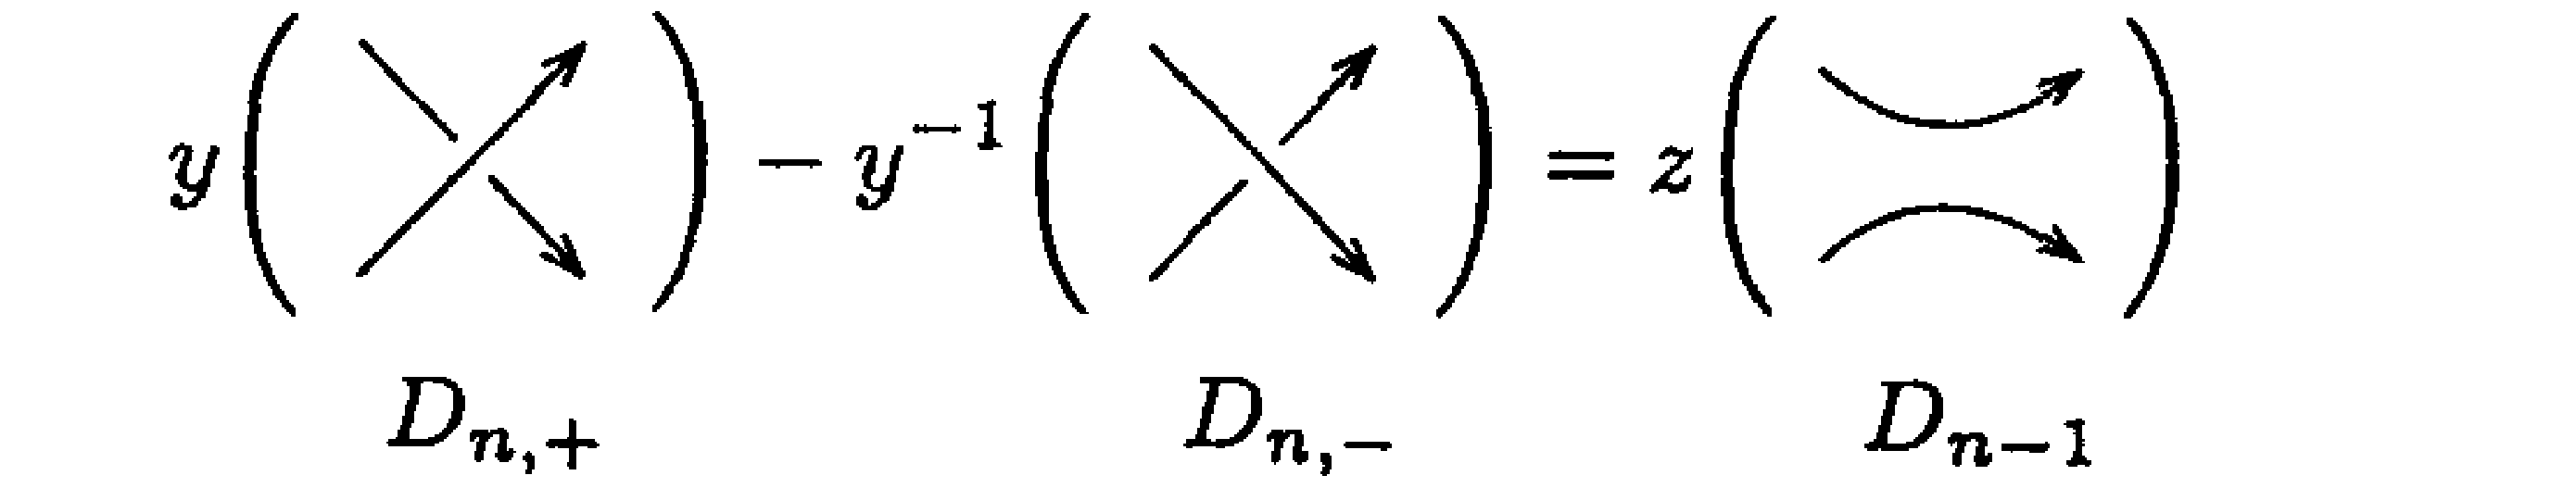
\includegraphics[width=0.95\textwidth]{figures/figA1.png}
\figtitle{A.1}{Alexander 多项式与 HOMFLY 多项式的定义}
\end{figure}

前两个图 $D_{n,\pm}$ 恰有 $n$ 个交叉，它们在屏幕上的投影完全相同；而且除一个交叉之外，二者的定向图完全重合。第三个图 $D_{n-1}$ 有 $n-1$ 个交叉（比另两个少一个）；其作法是把 $D_{n,\pm}$ 中任一个的、唯一与另一个相异的那个交叉的邻域，替换成图 A.1 所指示的、与定向自然相符的构型。相应各图的 Alexander 多项式之间有如下关系：
\[
zP_{D_{n-1}}(z)=P_{D_{n,+}}(z)-P_{D_{n,-}}(z).
\]
只要再补充如下条件，上式便可作为定义条件：任何具有 2 个或更多连通分量的图，其 Alexander 多项式为零；而平凡的单分支图（即简单闭曲线）的 Alexander 多项式等于 1。

% [Tutor Note: 这里用变量 $z$ 写出的正是 Conway 形式的 Alexander 多项式，$z=t^{1/2}-t^{-1/2}$，$t$ 为通常的 Alexander 变量。原书的初等定义只依赖「消去一个交叉」时的可加性，故须由上述两条补充条件把解定住：否则再加一个常数倍仍满足关系式，链环分量数不同的图之间也无从比较。]

% [原文 p.277]

这样就得到了作为变量 $z$ 的多项式的 Alexander 多项式；标准的写法再经一次代换得到：
\[
A(t,t^{-1})=P(z),\qquad z=t^{1/2}-t^{-1/2},
\]
最终得到 Alexander 多项式 $A(t,t^{-1})$，它在乘以 $t$ 的任意整数幂的意义下是良定义的。

\emph{HOMFLY 多项式} $H(x,y)$ 用同样的三个图定义，但采用更一般的条件
\[
xH_{D_{n-1}}(x,y)=yH_{D_{n,+}}(x,y)-y^{-1}H_{D_{n,-}}(x,y),
\]
再加上平凡纽结的 $H=1$ 这一条。注意：这类公式最一般的形式涉及三个变量，只要乘以一个适当的因子，便可约化为上述形状。

令 $y=1$、$x=z$ 就得到 Alexander 多项式；令 $x=y^{1/2}-y^{-1/2}$ 就得到著名的 \emph{Jones 多项式} $J(y)$，可见 HOMFLY 多项式是它的自然推广。下文把这些多项式（包括下面要定义的「Kauffman 多项式」）统称为 \emph{Jones 型多项式}。

现在叙述 Kauffman 的方法：它基于非定向图，构造出另一类多项式不变量，构成 Jones 多项式的另一种推广。如图 A.2 所示，有四个非定向图 $D_{n,\pm}$、$D_{n-1,1}$、$D_{n-1,2}$，它们只在一个交叉的小邻域内有差别；我们先由下述递推关系定义一个二元 \emph{状态多项式} $Q$：

\begin{figure}[htbp]
\centering
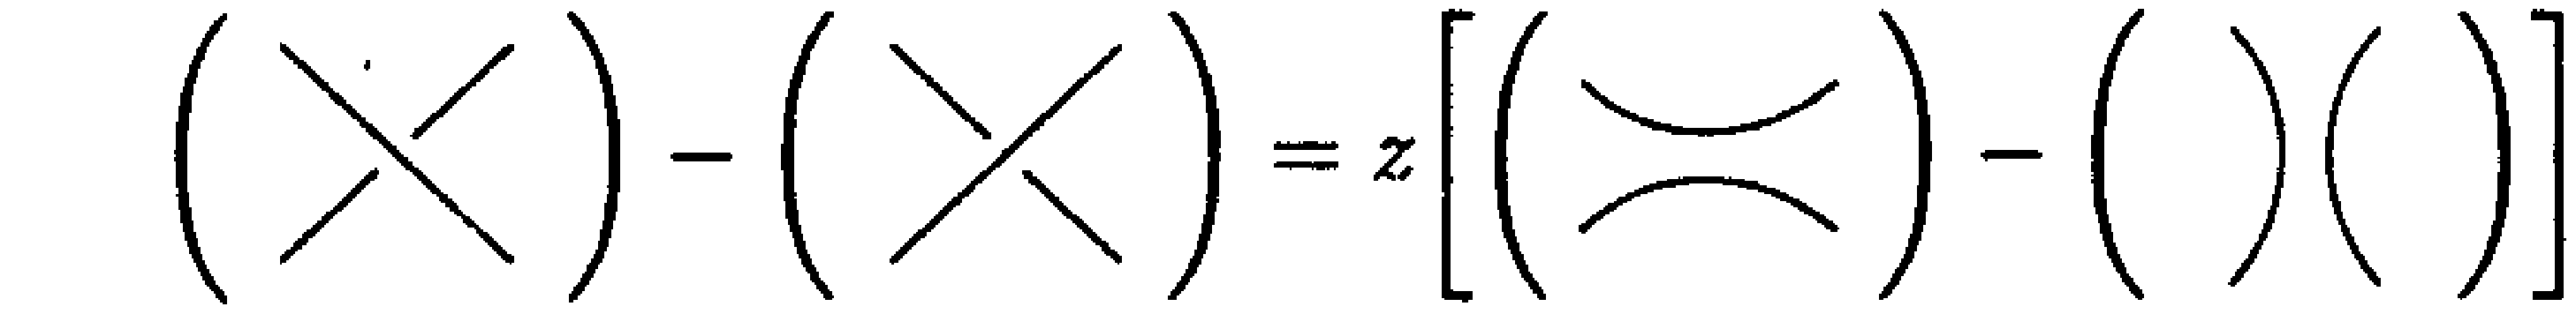
\includegraphics[width=0.9\textwidth]{figures/figA2.png}
\figtitle{A.2}{状态多项式与 Kauffman 多项式的定义}
\end{figure}

\[
Q_{D_{n,+}}-Q_{D_{n,-}}=z\bigl(Q_{D_{n-1,1}}-Q_{D_{n-1,2}}\bigr),
\]
并补充
\[
Q_{D_0}=\mu=\frac{a-a^{-1}}{z}+1
\]
其中 $D_0$ 是平凡的单分支图；同时要求：在每一次 Reidemeister 变换（见图 A.3）之下，$Q$ 改变一个因子 $a^{\pm 1}$。图 $D_n$ 的 \emph{Kauffman 多项式}随即定义为
\[
K_{D_n}=a^{-w(D_n)}Q_{D_n}(a,z),
\]
其中定向纽结或链环图 $D$ 的\emph{拧数}（writhe number）$w(D)$，定义为按各交叉的符号 $\pm 1$ 取代数和的量，符号的取法依

% [Tutor Note: 原书这一句把因子印作大写的 $A^{\pm 1}$，而同一段的 $Q_{D_0}=\mu(a,z)$、$K_{D_n}=a^{-w}Q_{D_n}(a,z)$ 皆用 $a$，故此处大字 $A$ 判为铅字误，正文统一写作 $a^{\pm 1}$。另「状态多项式」之名来自 Kauffman 的 state sum 模型：对图的每个交叉作两种光滑化求和，$Q$ 是这些状态权重的和。]

% [原文 p.278]

\begin{figure}[htbp]
\centering
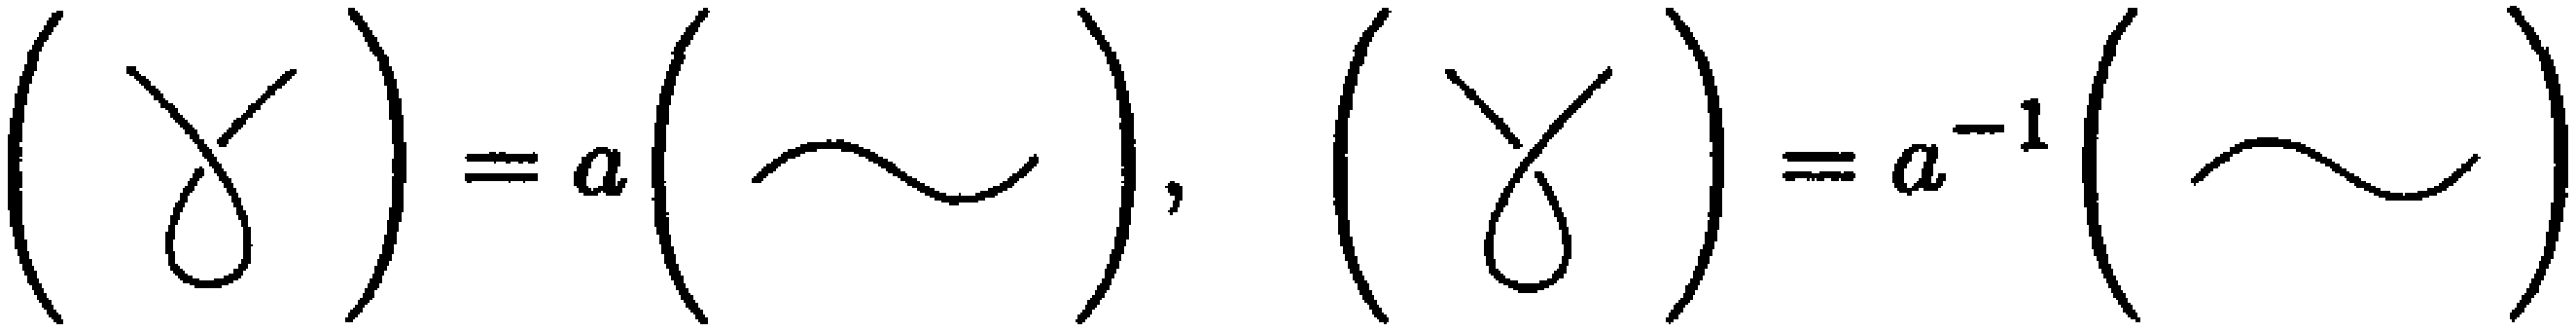
\includegraphics[width=0.92\textwidth]{figures/figA3.png}
\figtitle{A.3}{第一种 Reidemeister 变换与状态多项式}
\end{figure}

每个交叉处的符号依该交叉所决定的 2-标架的定向而定：标架的第一个向量取作（有向的）上支（见图 A.4）。（因此，图 $D$ 的定向只对拧数

\begin{figure}[htbp]
\centering
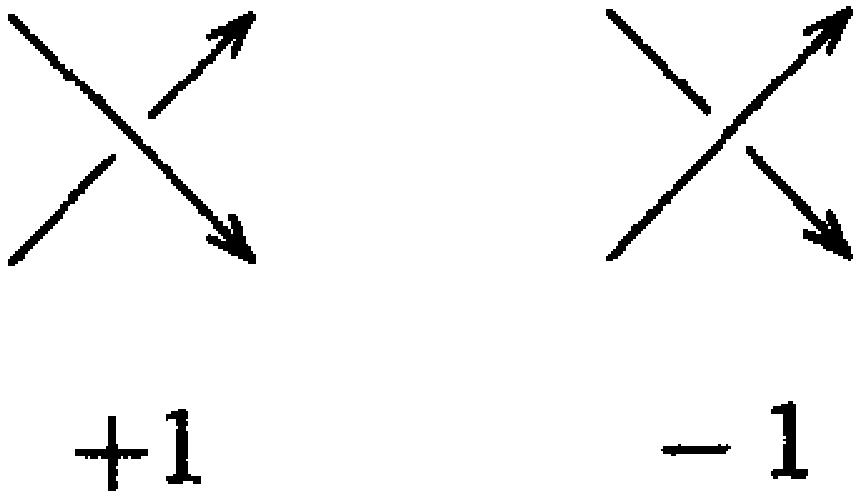
\includegraphics[width=0.62\textwidth]{figures/figA4.png}
\figtitle{A.4}{由交叉的定向决定的拧数}
\end{figure}

$w(D)$ 才有意义。）至此 Kauffman 多项式的定义完成；它是所论纽结或链环的不变量。

对任一有向图 $D$，$D$ 的 Jones 多项式随即由
\[
J_D(t)=\frac{K_D\bigl(z=t^{-1/4}-t^{1/4},\ a=t^{3/4}\bigr)}{t^{1/2}-t^{-1/2}}
\]
给出。另一方面，按 Jaeger 的一个定理，一个图的 Kauffman 多项式可以表示为与该图相联系的某些图的 HOMFLY 多项式的线性组合（系数取适当的数值）。

\begin{figure}[htbp]
\centering
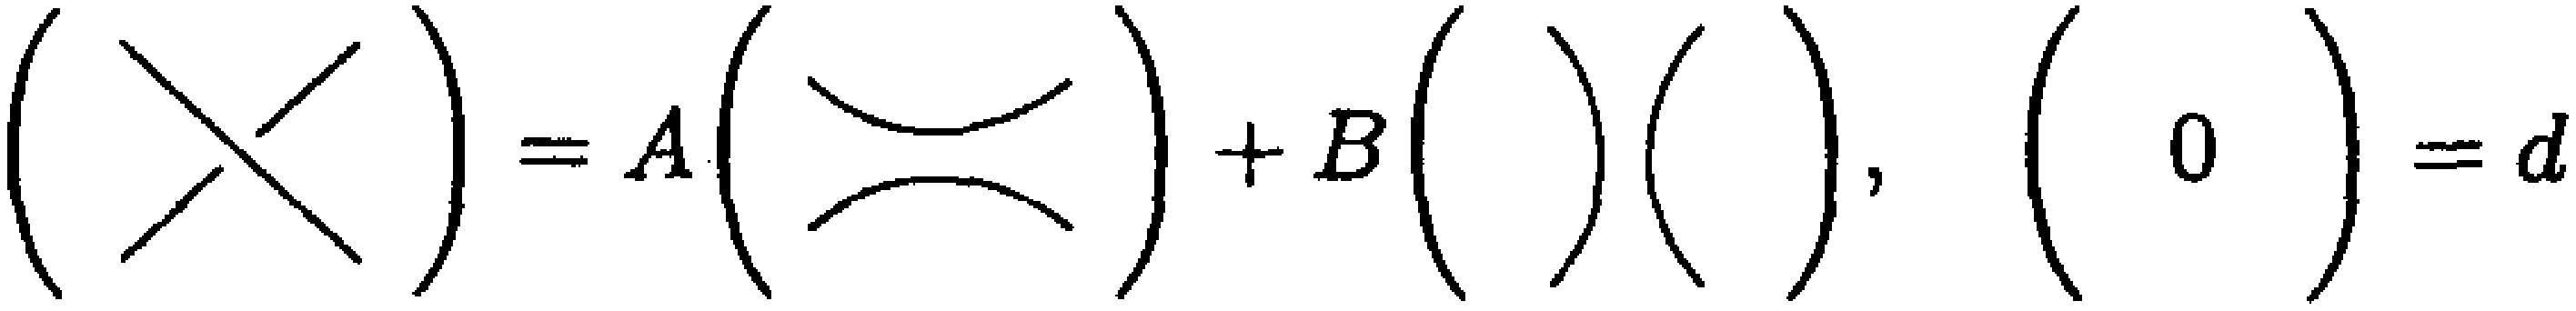
\includegraphics[width=0.95\textwidth]{figures/figA5.png}
\figtitle{A.5}{括号多项式与 Jones 多项式的定义}
\end{figure}

Kauffman 还通过递推关系定义了一个多项式 $S_{D_n}$（见图 A.5）：
\[
S_{D_n}(A,B;d)=AS_{D_{n-1,a}}+BS_{D_{n-1,b}},
\]
其中对平凡图 $D_0$ 取 $S_{D_0}=d$。作代换
\[
B=A^{-1},\qquad -d=A^2+A^{-2},
\]
便得到如下形式的 Jones 多项式：

% [Tutor Note: 这里的 $-d=A^2+A^{-2}$ 并非随意选取：括号多项式要满足第二种 Reidemeister 变换下的不变性，环数每增加一个就乘上 $d$，而两种光滑化权重之差恰须与 $d$ 相消，才迫使 $d=-A^2-A^{-2}$。原书随后给出的 $J_D(t)$ 公式，正是把 $K_D$ 沿 $z=t^{-1/4}-t^{1/4}$、$a=t^{3/4}$ 取值的特化，再除以 $t^{1/2}-t^{-1/2}$ 消去平凡分支的规范自由度。]

% [原文 p.279]

\begin{figure}[htbp]
\centering
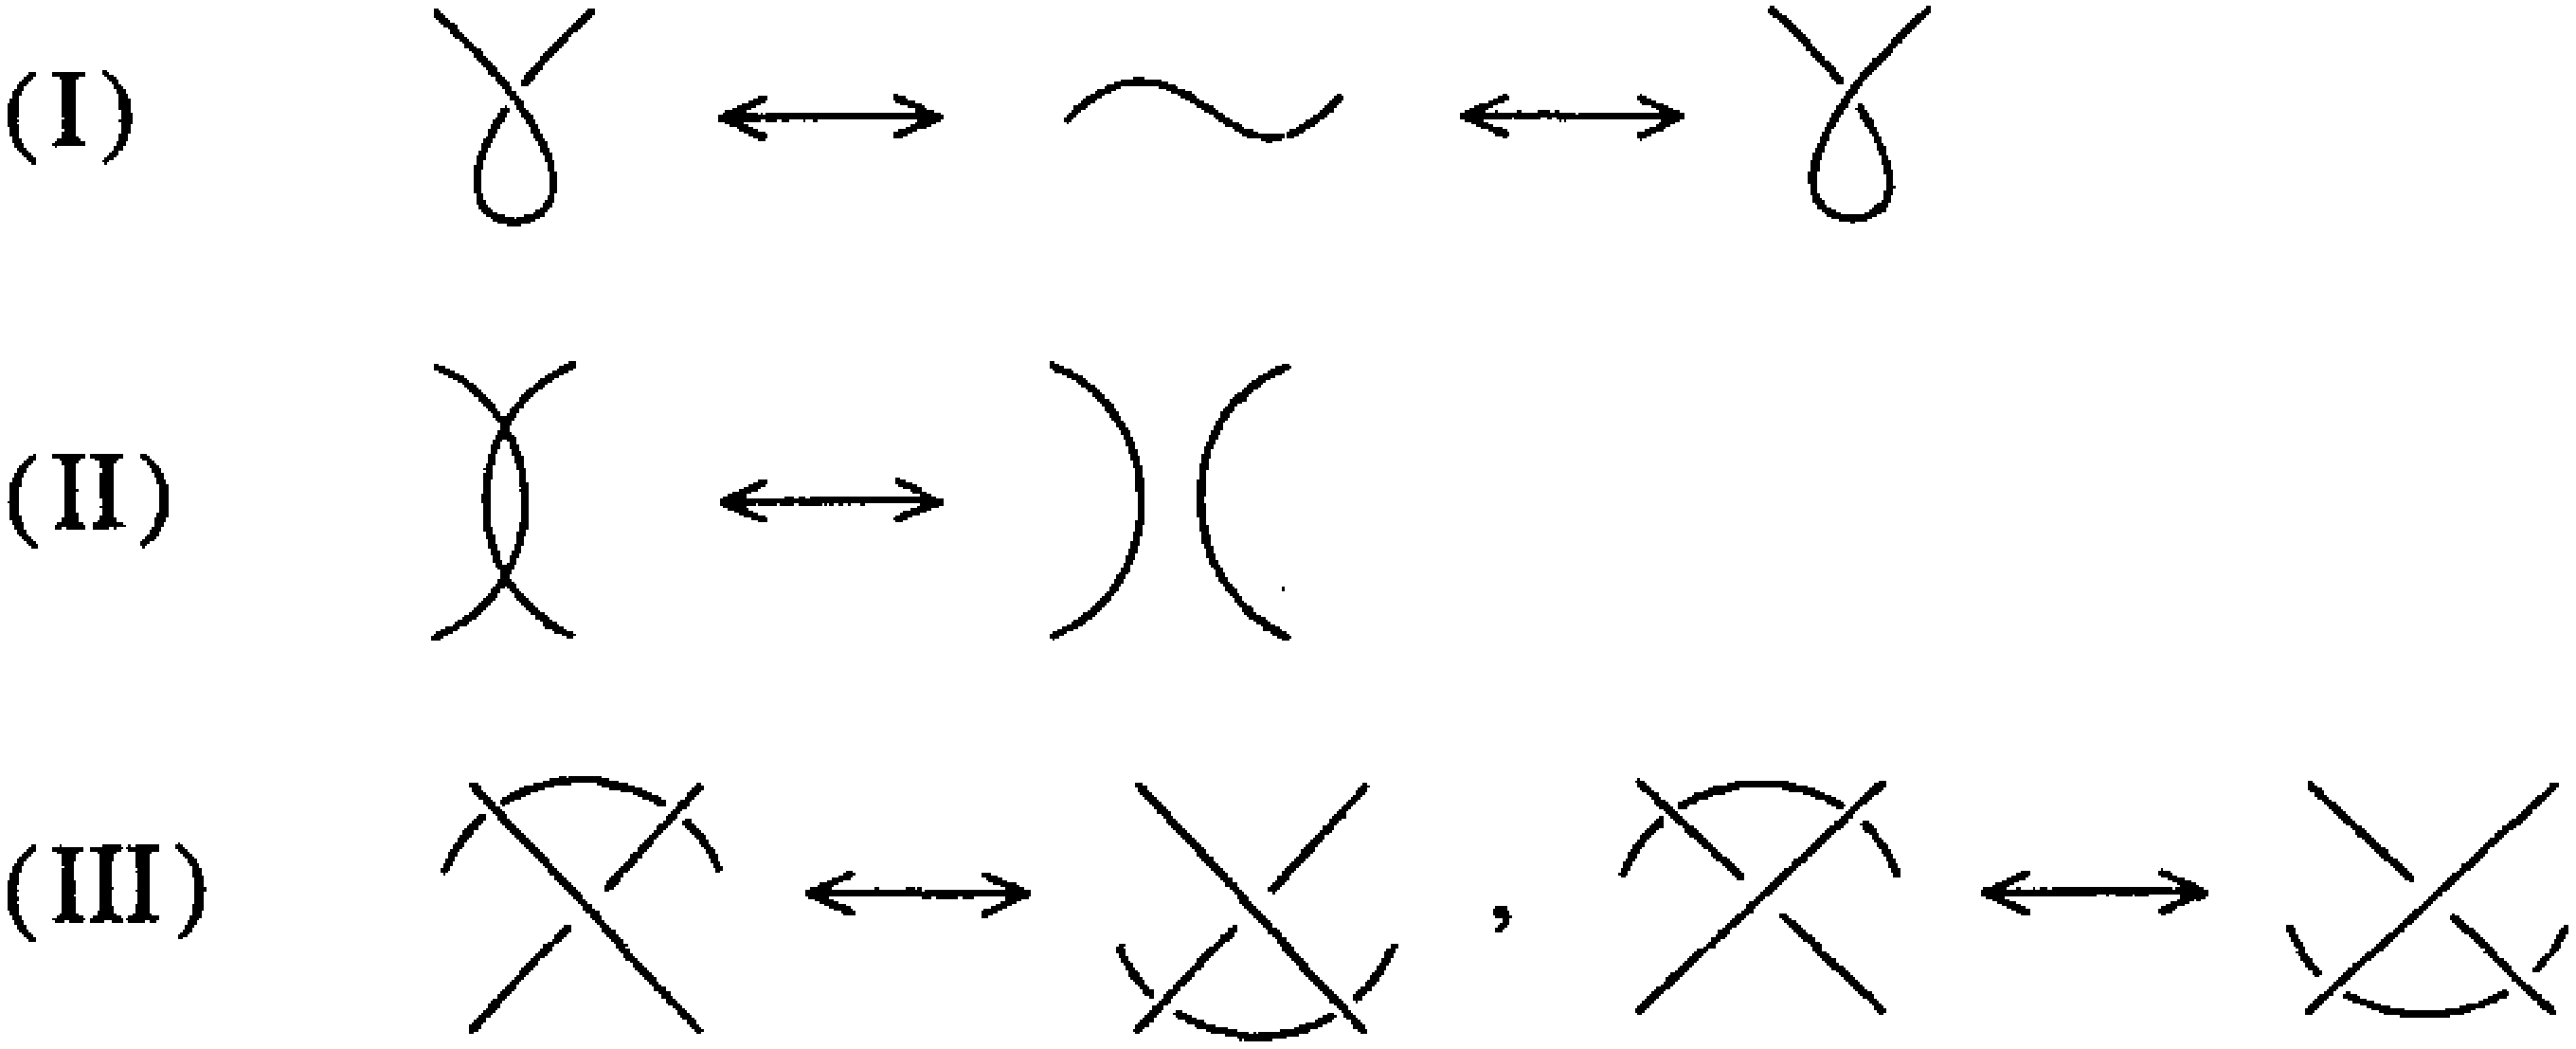
\includegraphics[width=0.88\textwidth]{figures/figA6.png}
\figtitle{A.6}{Reidemeister 变换}
\end{figure}

\[
J(A^4,A^{-4})=(-A)^{-3w(D)}S(A,B;d),\qquad t=A^{-4}.
\]

（下文用 Kauffman 的进路定义 3 维流形的 Turaev--Reshetikhin 不变量时，还会用到这里的「括号」多项式 $S$。）可见 Kauffman 提供了到达 Jones 多项式的两条不同途径。

上面所有这些多项式的拓扑不变性，都可以借助「Reidemeister 变换」以纯组合的方式建立起来；后者是图的三种类型的初等改变，实现纽结与链环的等价（见图 A.6）。

于是只需验证每个多项式在 Reidemeister 变换下不变；此后便可利用相应的递推关系来计算该多项式。（应当指出：在 Reidemeister 与 Markov 的时代（1930 与 1940 年代），把这些初等变换辨识出来并非平凡之事；而 Whitney、Pontryagin 与 Thom 引入「通有性质」这一概念（约自 1935 年至 1950 年代）之后，问题被简化到了对学生而言只是练习的程度：「取一个通有形变，把它分解为初等的拓扑变换。」）

在较早的纽结理论处理中（特别是 Dubrovin、Fomenko 与本书作者合著的《现代几何学》第二卷），Alexander 多项式的定义是用「群环中的微分」这一多少有悖直觉的运算来叙述的。（作者莫斯科讨论班上的 L. Alania 曾指出）这种「微分」可以沿如下拓扑途径得到：从纽结或链环 $K$ 在平面上的定向图出发，按标准方式算出纽结的群 $\pi_1(M)$（$M=S^3\setminus K$）的一个呈现，即对图的每条边给出一个生成元（见图 A.7），并对每个交叉给出一对关系。由于每一对关系中的一条不过是在说：与构成该交叉上支的两条边相应的两个生成元相等，所以这个呈现立即约化为生成元与关系个数都不变的那个标准呈现。恰有

% [原文 p.280]

\begin{figure}[htbp]
\centering
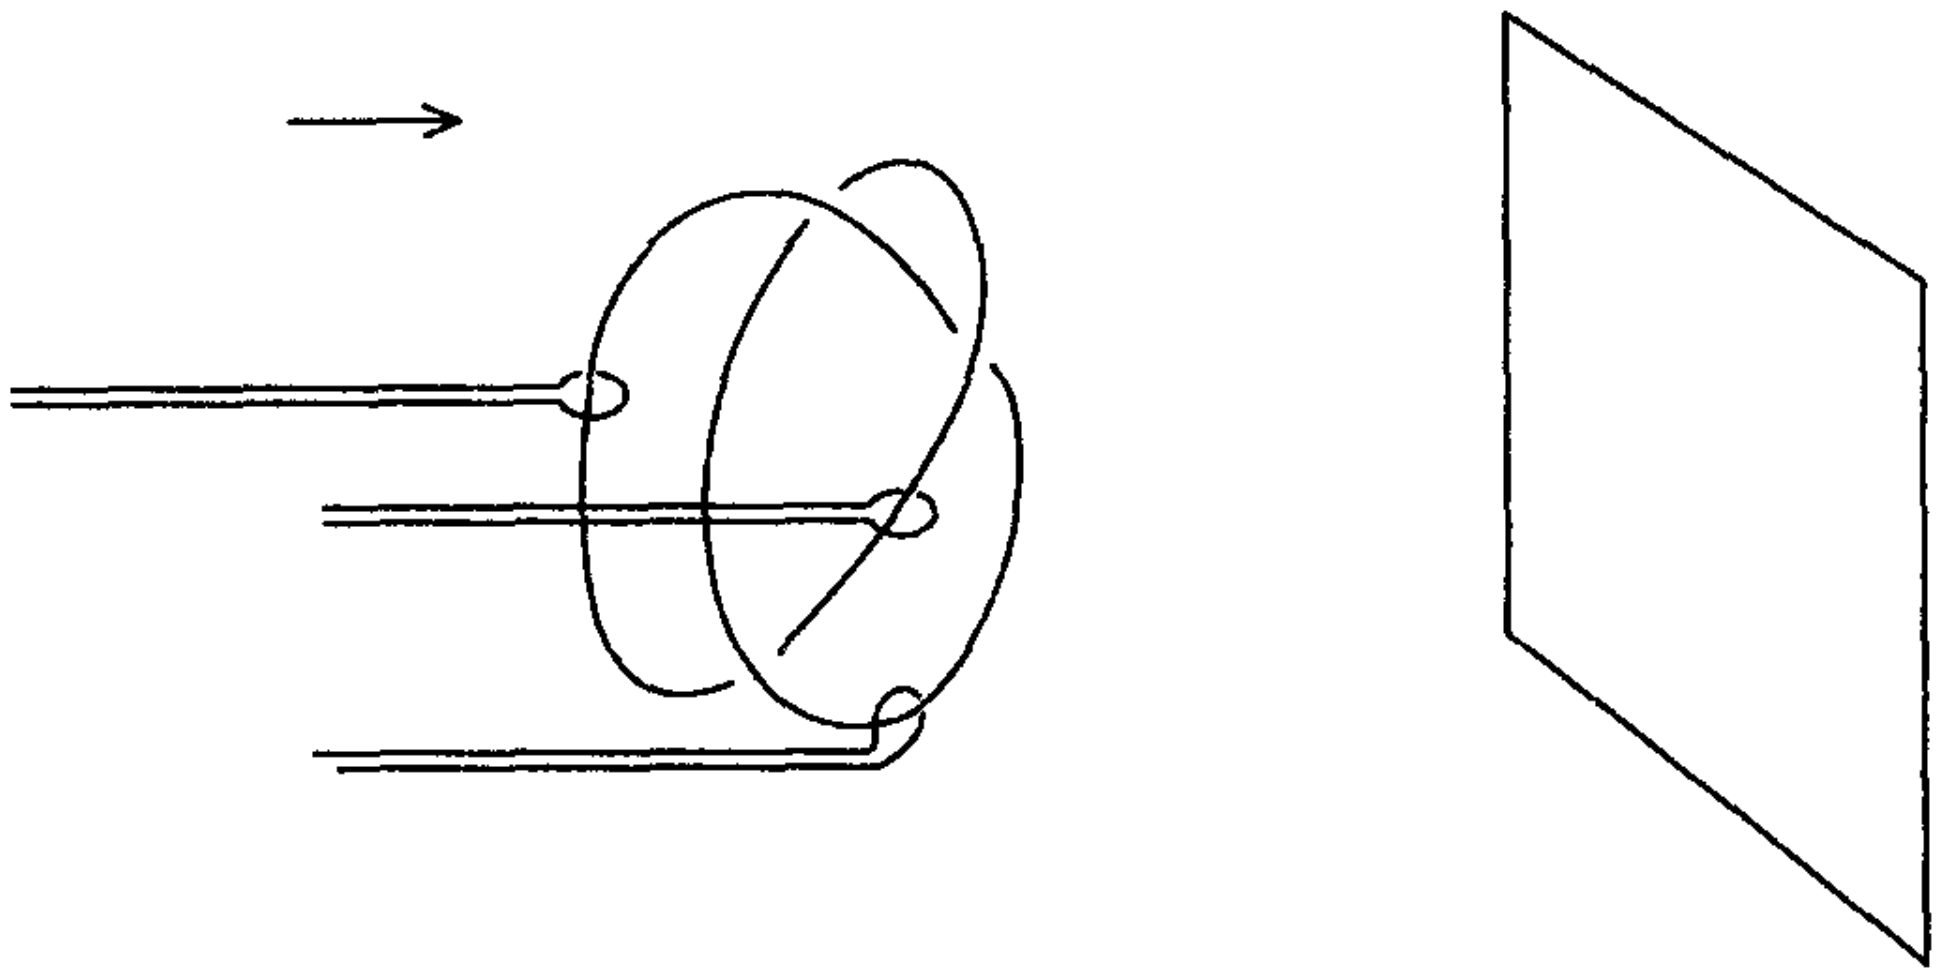
\includegraphics[width=0.80\textwidth]{figures/figA7.png}
\figtitle{A.7}{基本群的计算}
\end{figure}

一个 0-胞腔、以生成元标记的 1-胞腔、以关系标记的 2-胞腔构成的复形 $L$，随之是 $M$ 的形变收缩。提升到万有覆叠，便得到自由 $\Z[\pi_1]$-模复形上的一个边界算子；它表现为一个元素取自该群环的方阵，而与此前提到的「微分」相联系的正是这个矩阵，具体如下。记生成元为 $a_i$、关系为 $r_j$，定义算子 $\partial_{a_i}$ 为
\[
\partial_{a_i}(a_j)=\delta_{ij},\qquad
\partial_{a_i}(bc)=\partial_{a_i}(b)+b\partial_{a_i}(c);
\]
所论矩阵的元素 $q_{ij}$ 即由
\[
q_{ij}=\partial_{a_i}(r_j)
\]
给出。

% [Tutor Note: 这里的 $\partial_{a_i}$ 就是 Fox 自由微分：它对生成元取 $\delta_{ij}$，对乘积满足左导子法则（注意第二项中 $b$ 在左），正是「群环中求微分」的严格版本。它之所以对 Alexander 多项式有效，是因为它把 $\Z[\pi_1]$ 上的边界矩阵化为 $q_{ij}$ 这样的「抽象 Jacobi 矩阵」；Milnor 后来指出，Alexander 多项式本质上就是这一复形的挠率。]

把每个生成元 $a_i$ 映为 $t$，便得到整系数 Laurent 多项式环上的一个模复形，其边界算子就是相应的方阵，只是元素换成了 Laurent 多项式。这个矩阵的行列式为零，而其各代数余子式的最大公因式，在乘以 $t$ 的适当幂之后，恰好就是 Alexander 多项式 $A(t)$。

Milnor 在 1960 年代给出了 Alexander 多项式的同调论处理，用 $L$ 的 $\Z$-覆叠的一阶同调模（以 Euclid 环 $\Q[t,t^{-1}]$ 为系数环）的挠率来表述；他的讲法可沿上述路线给出。作者在 Soviet Math. Doklady 上的一则札记给出了如下更有吸引力的讲法。考虑一切一维表示 $\rho:\pi_1(M)\to\C$，以及以这种表示为局部系统数的同调 $H_i^\rho(M;\C)$。事实上，可以取 $M$ 为任意流形，把 $\C$ 换成 $\C^n$，并更一般地考虑 $\pi_1$ 在 $GL_n(\C)$ 中一切表示构成的空间 $\mathrm{Rep}_n(\pi_1)$——它是 $\Z$ 上的一个代数簇。同调群 $H_i^\rho(M;\C^n)$ 的秩 $b_i(\rho)$ 于是定义了该代数簇上的一个整值函数，它在几乎所有点处为常数（即在某些「跳跃」的代数子簇 $W_j\subset\mathrm{Rep}_n(\pi_1)$（定义在 $\Z$ 上）之外）；$b_i(\rho)$ 的值在每个这样的子簇上跳跃，在它们的两两交集上又进一步跳跃，如此递推。

% [原文 p.281]

在我们所考虑的特殊情形，即 $M=S^3\setminus K$（$K$ 为纽结）且 $n=1$ 时，得到的簇是 $\mathrm{Rep}_1(\pi_1)=\C\setminus\{0\}=\C^*$。此时有如下结果：

\begin{quote}
\itshape
当 $i=1$ 时，跳跃子簇构成一个有限点集，而它恰好就是 Alexander 多项式的根集。
\end{quote}

% [Tutor Note: 这条断言把 Alexander 多项式的根解释为表示簇 $\C^*=\mathrm{Hom}(\pi_1,\C^*)$ 上的跳跃点：对一维表示 $\rho$，局部系统数同调 $H_1^\rho$ 的维数在 $\rho$ 走到 $A(t)=0$ 的根处发生跳跃。这正是「Alexander 多项式是基本群的一维表示簇的跳跃轨迹」这一现代观点的雏形。]

对于有 $k$ 个分支的链环，有 $H_1(M)=\Z^k$ 与 $\mathrm{Rep}_n(\pi_1)=(\C^*)^k$，于是得到相应的跳跃子簇，以及 $k$ 个变量的「广义 Alexander 多项式」。多变量 Alexander 多项式的一种现代初等组合处理，是 H. Murakami 几年前给出的。

这幅图景中的代数几何是同伦不变的，但可能相当复杂；即便在 $M=S^3\setminus K$（$K$ 为链环）的情形，也仍未被很好地理解。

本书作者曾猜想：当 $n=2$ 时，应当能从跳跃子簇的结构直接提取出 Jones 多项式与 HOMFLY 多项式。然而几年前 Le Tu 在莫斯科考察了二桥纽结这一有趣情形下的这些子簇，发现其结构远比预期的复杂。因此，寻找 Jones 多项式的经典代数-拓扑处理这一问题，至今仍未解决。

下面给出 Alexander、Jones 与 HOMFLY 多项式的第三种定义，它用到辫群 $B_n$。先回忆这些群的定义。

考虑由生成元 $\sigma_i$（$i\in\Z$）与关系
\[
\sigma_i\sigma_j=\sigma_j\sigma_i,\quad |i-j|>1;\qquad
\sigma_i\sigma_{i+1}\sigma_i=\sigma_{i+1}\sigma_i\sigma_{i+1}
\]
给出的群。

第 $n$ 个\emph{辫群} $B_n$ 随即是由 $n$ 个相继的生成元 $\sigma_{k+1},\dots,\sigma_{k+n}$ 所生成的子群。于是有 $B_n$ 到 $B_{n+1}$ 的自然嵌入。（更标准的做法是取 $B_n$ 为由 $\sigma_1,\dots,\sigma_n$ 生成的子群，即取 $k=0$。）

按 Markov（Jr.）在 1940 年代的一个定理，纽结与链环的等价类之集，与辫在由下述两种初等运算（\emph{Markov 变换}）所确定的等价关系下的等价类之集，成自然的一一对应：

\begin{enumerate}
\item 用任意元素 $c\in B_n$ 共轭任一辫 $a\in B_n$：$a\sim cac^{-1}$；
\item 用 $\sigma_{n+1}^{\pm 1}\in B_{n+1}$ 右乘任一辫 $a\in B_n$：$a\sim a\sigma_{n+1}^{\pm 1}$。
\end{enumerate}

两个辫称为\emph{等价}的，如果其中之一能借有限多个初等 Markov 变换化为另一个。

% [Tutor Note: 这里的 Markov 是小马尔可夫（A. A. Markov Jr.），与概率论中的 Markov 链无关；他在 1930 年代用辫群给出了纽结与链环的分类，即把几何问题化归为辫群的代数问题。注意原文把第二种运算写成右乘 $\sigma_{n+1}^{\pm 1}$，而它实际上在 $B_{n+1}$ 中进行——辫的「稳定化」与「去稳定化」由此进入等价关系。]

% [原文 p.282]

这一对应背后的想法既简单又自然。考虑 $\R^3$ 中由 $x^2+y^2=1$、$z=0$ 给出的圆周 $S^1$，以及它的小半径管状邻域 $T$：$\R^3\supset T\supset S^1$。所谓\emph{横截的}纽结或链环，就定义为 $T$ 中的一条简单闭曲线（或若干条这样的曲线），其切向量处处横截于与圆周正交的 2-球面。把管状邻域沿圆周在任一点处正交切开，便由横截纽结或链环得到辫。事实上，最先证明 $\R^3$ 中任何纽结或链环都同痕于横截纽结或链环的正是 Alexander；Markov 修正了他论证中的一处缺陷。

第 $n$ 个辫群 $B_n$ 在 $GL_n(A)$ 中的任一线性表示 $\rho$（$A$ 为任意交换结合环）都有特征标（迹函数），它在上述第一种初等 Markov 运算下不变：
\[
\chi_\rho(a)=\Tr[\rho(a)],\qquad a\in B_n.
\]

为了从一开始就得到这样的表示（而且对所有 $n$ 同时得到），可以试着用满足上述定义关系的矩阵来表示生成元 $\sigma_i$（$i\in\Z$）。Jones 借助求解统计物理与量子场论中某些可积模型的技巧，以这种方式得到了这样一类表示；他由此从 Yang--Baxter 方程出发，得到了一切辫群同时适用的、特殊的一类「局部、平移不变」的表示。

设 $V$ 是向量空间，
\[
S:V\otimes V\to V\otimes V
\]
是线性变换，具有如下性质：在 $V$ 的三份拷贝的张量积 $V\otimes V\otimes V$ 上，有
\[
S_{12}S_{23}S_{12}=S_{23}S_{12}S_{23},
\]
其中 $S_{ij}$ 在 $V\otimes V\otimes V$ 中第 $i$ 与第 $j$ 份拷贝的张量积上与 $S$ 相同，在其余拷贝上则限制为恒等映射。（注意：在可解统计模型的理论中，Yang--Baxter 方程常写得更一般，即对形如 $R=\tau S$ 的映射写出，其中 $S:V_i\otimes V_j\to V_i\otimes V_j$，$\tau:v_i\otimes v_j\mapsto v_j\otimes v_i$ 是置换映射；而此时 $V_i\otimes V_j\otimes V_k$ 的三个因子可以互不相同。）此时方程的形式为
\[
R_{12}R_{13}R_{23}=R_{23}R_{13}R_{12}.
\]

定义
\[
\rho(\sigma_i)=S_{i,i+1},
\]
便得到无穷辫群在可数多份 $V$ 的无穷张量积上的线性变换表示 $\rho$；它限制为第 $n$ 个辫群 $B_n$ 在空间 $V\otimes V\otimes\cdots\otimes V$（$n+1$ 个因子）上的线性变换表示 $\rho_n$。于是每个

% [Tutor Note: 这段构造解释了为什么 Jones 多项式能从辫群得出：辫的闭包给出链环，而第一种 Markov 变换（共轭）下迹函数不变；第二种变换要不变，就必须用一个在张量幂上相容的「Markov 迹」（即把 $S^{\pm 1}$ 乘进去再取迹），Jones 的技巧正在于此。原书取 $n+1$ 个因子，是因为 $B_n$ 的生成元 $\sigma_1,\dots,\sigma_n$ 中最后一个 $\sigma_n$ 要作用在第 $n$ 与第 $n+1$ 份拷贝上。]

% CHUNK appa DONE
